\documentclass[twocolumn, 12pt]{article}

\usepackage[utf8]{inputenc}
\usepackage[english, spanish]{babel}
\usepackage{fullpage} % changes the margin
\usepackage{graphicx}
\usepackage{amsmath}
\usepackage{enumitem}
\usepackage{chngcntr}
\usepackage{setspace}
\usepackage{url}
\usepackage{csquotes}
\usepackage{float}
\usepackage{verbatim}
\usepackage{tabularx}
\usepackage{amsmath}

\counterwithin{figure}{section}
\renewcommand{\thesection}{\arabic{section}}
\renewcommand{\thesubsection}{\thesection.\arabic{subsection}}
\renewcommand{\baselinestretch}{2}

\usepackage[style=apa, maxnames=6, minnames=3, backend=biber]{biblatex}
\DefineBibliographyStrings{english}{%chktex-file 1 chktex-file 6
	andothers = {\em et\addabbrvspace al\adddot}
}
\addbibresource{./Bibliography/bibliography.bib}

\begin{document}

\begin{titlepage}
      \centering
      
\includegraphics[width=0.3\textwidth]{Images/logo_utb.png}\par\vspace{1cm}
      {\scshape\LARGE Universidad Tecnológica de Bolívar \par}
      \vspace{.5cm}

      {\scshape\Large Introducción a log negocios internacionales \par}
      \vspace{.2cm}

      % chktex-file 8
      \slshape {\Large \bfseries{}Trabajo Investigativo\\}
      \slshape {\small \bfseries{}NVIDIA y su relación con el mercado Taiwanés}
      \vspace{1cm}

      \slshape {\itshape{} Valentina Del Rio \\}
      \slshape {\itshape{} Juliana Arias \\}
      \slshape {\itshape{} Valentina Niño \\}
      \slshape {\itshape{} Maria Grau \\}
      \slshape {\itshape{} Valeria Santamaria \\}
      \vfill
      Revisado Por \\
      Javier Mauricio Prieto \\
      {\large \today\par}
\end{titlepage}

% chktex-file 44
% chktex-file 24

\nocite{*}

\section{Introducción}

NVIDIA Corporation, fundada en 1993 por Jen-Hsun Huang, Chris
Malachowsky y Curtis Priem en Santa Clara, California, es una
empresa líder en tecnología que ha dejado una huella
significativa en la industria de la informática y la
inteligencia artificial. Se especializa en el diseño y
desarrollo de unidades de procesamiento de gráficos (GPU),
así como en soluciones de inteligencia artificial.

NVIDIA es conocida por su innovación en las GPU.~Estas unidades
son esenciales para el procesamiento gráfico en computadoras
personales, estaciones de trabajo y servidores, revolucionando
los gráficos en videojuegos, diseño 3D, simulaciones científicas
y más.

La empresa también ha desempeñado un papel fundamental en
el avance de la inteligencia artificial. Sus GPU se utilizan
en tareas de aprendizaje profundo y procesamiento de datos
masivos; ha desarrollado bibliotecas y herramientas que
permiten a los investigadores y desarrolladores aprovechar
la potencia de la IA.\@{}

\section{Historia}

NVIDIA, una empresa líder en tecnología de procesamiento gráfico
ha tenido un gran impacto en la industria desde que fue fundada
en 1993 en Silicon Valley, California. En sus primeros años,
NVIDIA se enfocó en desarrollar soluciones gráficas para
computadoras personales, previendo la creciente necesidad de
gráficos avanzados en el mercado emergente de los videojuegos.

En 1999, NVIDIA marcó un hito significativo en la historia de la
industria con el lanzamiento de su GPU GeForce 256. NVIDIA se
estableció como líder en rendimiento gráfico gracias a la
introducción de esta revolucionaria GPU con capacidades sin
precedentes.

Una empresa líder en el mercado de tarjetas gráficas. Desde ese
momento, la empresa ha continuado innovando y ampliando su alcance,
incursionando en campos como la inteligencia artificial, el cómputo
de alto rendimiento y la conducción autónoma.

La introducción de la arquitectura CUDA en 2006 fue un momento
crucial en la historia de NVIDIA, ya que permitió a las GPUs
llevar a cabo tareas de computación general, abriendo nuevas posibilidades en campos como la ciencia, la investigación y el aprendizaje profundo.

NVIDIA ha lanzado innovaciones recientes, como la arquitectura
Turing en 2018, que trajo tecnologías avanzadas como el trazado
de rayos en tiempo real y el aprendizaje profundo acelerado por
GPU.~La serie GeForce RTX 30, lanzada en 2020,
estableció nuevos estándares de rendimiento gráfico para
juegos y aplicaciones de creación de contenido, consolidando
aún más el liderazgo de NVIDIA en la industria.

Su historia, tal como se presenta en su línea de tiempo
corporativa, abarca varias décadas de innovación y avances
en la industria de la tecnología, desde 1993 hasta el 2020
desde su fundación.

\begin{figure}[H]
      \begin{center}
            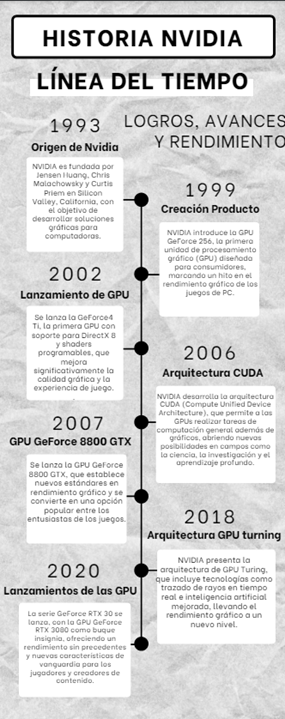
\includegraphics[width=.5\linewidth]{./Images/LineaTiempo.png}
            \caption{Linea de tiempo de NVIDIA}
      \end{center}
\end{figure}

\section{Objetivos y vision de la empresa}

La compañía NVIDIA Corporation es reconocida por ofrecer soluciones
en gráficos, computación y redes a nivel global. La oferta incluye
productos como las tarjetas gráficas GeForce, perfectas para
jugadores y usuarios de PC, y el servicio de transmisión de
juegos GeForce NOW.~Además, ofrecen soluciones para
profesionales, como las GPU Quadro/NVIDIA RTX, que se
utilizan en estaciones de trabajo para tareas gráficas
exigentes. También ofrecen una variedad de productos
para centros de datos y redes, como plataformas
informáticas y de redes, y se especializan en el área
de la conducción automatizada con su plataforma NVIDIA DRIVE.\@{}

Los videojuegos, la visualización profesional, los centros
de datos y la industria automotriz son algunos de los
principales sectores que se benefician de los productos de NVIDIA.~La
compañía vende sus productos a varios tipos de clientes,
como fabricantes de equipos originales, distribuidores y
proveedores de servicios en la nube.

\section{Marco Teorico}

\subsection*{Posicionamiento de NVIDIA en el mercado de tecnología y GPU}

\begin{itemize}
      \item Revisión de literatura sobre la evolución de NVIDIA
            como líder en el mercado de procesamiento gráfico (GPU) y
            tecnologías relacionadas.

      \item Análisis de las estrategias de marketing,
            investigación y desarrollo que han contribuido al éxito de
            NVIDIA en el mercado.

      \item Exploración de la relación entre la innovación
            tecnológica, la calidad del producto y la percepción de la
            marca en la posición competitiva de NVIDIA.\@{}
\end{itemize}

\subsection*{Mercados más y menos significativos para NVIDIA}

\begin{itemize}
      \item Identificación y análisis de los mercados verticales más
            importantes para NVIDIA, como la inteligencia artificial, los
            videojuegos, la computación en la nube, el automóvil autónomo
            y la visualización profesional.

      \item Evaluación de oportunidades y desafíos en cada mercado,
            incluyendo factores económicos, regulatorios y tecnológicos.

      \item Investigación de los mercados emergentes y nichos
            de mercado que podrían ofrecer nuevas oportunidades de
            crecimiento para NVIDIA, así como los mercados que pueden
            estar disminuyendo en importancia.
\end{itemize}

\subsection*{Relación entre NVIDIA y el mercado Taiwanés}

\begin{itemize}
      \item Examen de la colaboración histórica entre NVIDIA y las
            empresas taiwanesas en la fabricación de componentes
            electrónicos, como chips de GPU y tarjetas gráficas.

      \item Análisis de la integración vertical y horizontal de la
            cadena de suministro de NVIDIA en Taiwán, incluyendo
            relaciones con fabricantes de semiconductores,
            ensambladores de tarjetas gráficas y otros proveedores de
            tecnología.

      \item Investigación de las políticas gubernamentales,
            las condiciones económicas y las dinámicas empresariales en
            Taiwán que pueden afectar la relación entre NVIDIA y el mercado
            taiwanés.
\end{itemize}

\subsection*{Implicaciones para el futuro de NVIDIA}

\begin{itemize}
      \item Discusión de las oportunidades estratégicas y los riesgos
            potenciales que enfrenta NVIDIA en el contexto de su posición
            en el mercado y sus relaciones con Taiwán y otros mercados clave.

      \item Propuesta de recomendaciones para NVIDIA basadas en
            las tendencias identificadas en la investigación, incluyendo
            áreas de expansión, colaboración empresarial y gestión de riesgos.
\end{itemize}

\section{Posición en el mercado}

NVIDIA es líder en varios mercados clave, incluidos los videojuegos,
la inteligencia artificial, la computación de alto rendimiento y
la automoción. Su dominio en estos sectores le proporciona una
posición sólida en la industria de la tecnología y le permite
influir en la dirección futura de la misma

En el primer trimestre de 2024, Nvidia fue responsable del
11.02\% del rendimiento del índice de rendimiento total
del S\&P 500, seguido por Microsoft con un 3.69\%, Meta
con un 3.20\% y Amazon con un 2.83\%; lo que nos permite
decir que Nvidia ha sido el contribuyente más crítico a las
ganancias del mercado en 2024.

La posición económica de NVIDIA es bastante sólida y ha sido
así durante varios años y esto se refleja en sus estados financieros.

Ingresos y crecimiento: NVIDIA ha experimentado un crecimiento
constante en sus ingresos a lo largo de los años, impulsado por
su liderazgo en tecnologías de procesamiento gráfico (GPU) y
su expansión hacia áreas como inteligencia artificial, centros
de datos y automoción. Su capacidad para diversificar sus ingresos
ha contribuido a un crecimiento estable y significativo.

Rentabilidad: esta empresa ha mantenido márgenes de ganancia
saludables, lo que indica su eficiencia operativa y su capacidad
para generar beneficios a partir de sus operaciones comerciales.
Esto ha sido respaldado por su enfoque en productos de alto
rendimiento y soluciones tecnológicas innovadoras.

Balance financiero: NVIDIA tiene un balance financiero sólido,
con una posición de efectivo estable y una gestión prudente de
la deuda. Esto le proporciona flexibilidad financiera para
invertir en investigación y desarrollo, realizar adquisiciones
estratégicas y realizar recompras de acciones para generar valor
para los accionistas.

\begin{figure}[H]
      \begin{center}
            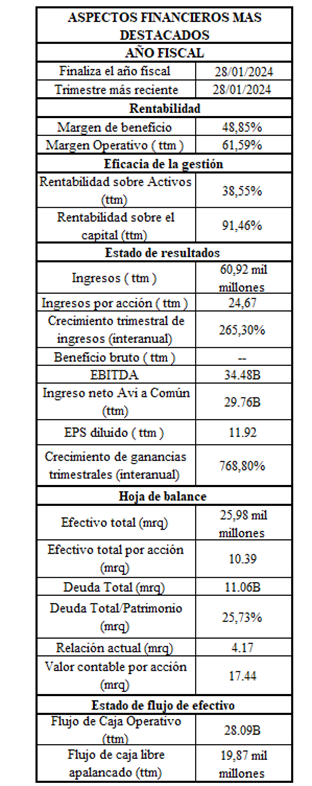
\includegraphics[width=\linewidth]{./Images/Anexo2.png}
            \caption{}
      \end{center}
\end{figure}

\subsubsection*{Mercados más significativos para NVIDIA}

\begin{itemize}
      \item Estados Unidos:
            NVIDIA tiene su sede en Santa Clara, California,
            Estados Unidos. Aquí se hace gran parte de su investigación,
            desarrollo y operaciones.

      \item Taiwán:
            Taiwán es un país importante para NVIDIA debido a su
            papel en la fabricación de componentes electrónicos.
            NVIDIA tiene una presencia significativa en Taiwán,
            especialmente en el ámbito de las GPU y la tecnología.

      \item China:
            China es un mercado crucial para NVIDIA debido a su
            tamaño y crecimiento económico. La empresa tiene
            operaciones y colaboraciones en China para atender a
            la creciente demanda de tecnología.

      \item Japón:
            Japón es un país líder en tecnología y un mercado
            importante para NVIDIA.~La empresa trabaja con socios
            japoneses en áreas como la inteligencia artificial,
            la robótica y la computación de alto rendimiento.

      \item Alemania:
            Alemania es un centro tecnológico en Europa y un
            mercado estratégico para NVIDIA.~La empresa colabora
            con instituciones académicas y empresas alemanas en
            proyectos de investigación y desarrollo.

      \item Reino Unido:
            NVIDIA tiene una presencia significativa en el Reino
            Unido, especialmente en áreas como la inteligencia
            artificial, la visualización profesional y la computación
            de alto rendimiento.

      \item India:
            India es un mercado emergente con un gran potencial
            para NVIDIA.~La empresa tiene oficinas y colaboraciones
            en India para atender a las necesidades tecnológicas del país.

      \item Francia:
            Francia es otro país europeo importante para NVIDIA.~La
            empresa trabaja con socios franceses en proyectos
            de investigación, desarrollo y aplicaciones tecnológicas.

\end{itemize}

\subsection*{Mercados menos significativos para NVIDIA (no tiene lazos comerciales):}

\begin{itemize}
      \item Singapur:
            Aunque Singapur es un país pequeño, ha desempeñado un
            papel importante en el éxito de NVIDIA.~En el tercer trimestre de
            ventas de 2023, Singapur ocupó el cuarto lugar en los rankings de ventas
            de NVIDIA, contribuyendo al 15% de sus ingresos. Esto se debe en parte a su enfoque en el procesamiento de datos y la tecnología.

      \item Emiratos Árabes Unidos (EAU):
            Aunque EAU no es un mercado central
            para NVIDIA, no se menciona con frecuencia como un destino importante
            para la empresa. Sin embargo, su enfoque en la inteligencia artificial y
            la tecnología podría cambiar esto en el futuro.

      \item Holanda (Países Bajos):
            Aunque Holanda es favorable para
            emprendedores, no se destaca como un mercado crucial para NVIDIA.~Sin
            embargo, su economía fuerte y políticas empresariales sólidas podrían
            atraer más atención en el futuro.

      \item Finlandia:
            A pesar de ser un centro tecnológico, Finlandia no se
            menciona ampliamente como un mercado clave para NVIDIA.~Sin embargo,
            su enfoque en la educación empresarial y la innovación podría
            cambiar esta percepción.

      \item Canadá:
            Aunque Canadá es un país tecnológicamente avanzado, no se
            considera uno de los mercados más relevantes para NVIDIA.~Sin embargo, su
            comunidad de investigación y desarrollo sigue siendo un activo importante.

\end{itemize}

\section{Innovación tecnológica}

NVIDIA es reconocida por su innovación en tecnología de GPU y su
capacidad para desarrollar soluciones avanzadas que impulsan el
progreso en varias industrias. Esta capacidad para innovar y
mantenerse a la vanguardia de la tecnología contribuye a su
fortaleza económica y competitiva.

\begin{itemize}
      \item GPU para videojuegos:
            NVIDIA ha sido pionera en el desarrollo de GPUs de alto rendimiento
            para la industria de los videojuegos. Sus tarjetas gráficas GeForce
            son reconocidas por su potencia, rendimiento y calidad de gráficos,
            lo que ha contribuido mucho a avanzar en los gráficos de videojuegos
            y a la experiencia de juego inmersa.

      \item Computación de alto rendimiento (HPC):
            NVIDIA ha desarrollado GPUs especializadas para aplicaciones de HPC,
            permitiendo un procesamiento masivo de datos y un rendimiento
            excepcional en aplicaciones científicas, de investigación y de
            análisis de datos. Su arquitectura CUDA
            (Compute Unified Device Architecture) ha sido fundamental en este
            ámbito.

      \item Inteligencia Artificial (IA) y Aprendizaje Automático (ML):
            NVIDIA ha ampliado su enfoque más allá de los gráficos para
            convertirse en un jugador importante en el campo de la IA y
            el ML.~Sus GPUs aceleradoras, como la serie NVIDIA Tesla y las
            unidades de procesamiento tensorial (TPU), son ampliamente utilizadas
            en aplicaciones de entrenamiento y ejecución de modelos de IA/ML.\@{}

      \item Centros de datos y computación en la nube:
            NVIDIA ha desarrollado soluciones específicas para aplicaciones
            en centros de datos y entornos de computación en la nube. Sus
            GPUs Tesla y su plataforma de computación NVIDIA DGX son
            utilizadas por empresas y proveedores de servicios en la nube para
            acelerar el procesamiento de datos y el entrenamiento de modelos
            de IA a escala.

      \item Automoción:
            NVIDIA ha incursionado en el mercado automotriz con su plataforma
            NVIDIA DRIVE, que ofrece soluciones avanzadas de procesamiento
            de datos para vehículos autónomos y sistemas de asistencia al
            conductor. Su tecnología se utiliza en sistemas de conducción
            autónoma de nivel 2 a nivel 5, así como en sistemas de
            infoentretenimiento y visualización avanzada.

      \item Realidad Virtual y Aumentada:
            NVIDIA ha desarrollado tecnología para impulsar experiencias
            inmersivas de realidad virtual (VR) y aumentada (AR). Sus GPUs
            y software están presentes en dispositivos de VR/AR de alta gama,
            lo que permite gráficos de alta calidad y un rendimiento fluido
            en aplicaciones de entretenimiento, diseño y formación.

\end{itemize}

\section{Análisis de la relación entre NVIDIA y el mercado Taiwanés}

Taiwán desempeña un papel crucial en la cadena de suministro
global de NVIDIA, principalmente debido a su sólida
infraestructura en la industria de semiconductores. La isla
alberga algunas de las fábricas más avanzadas del mundo, como
las de Taiwán Semiconductor Manufacturing Company (TSMC), que
es un socio clave para NVIDIA.\@{}

\subsection*{Lazos históricos de NVIDIA}

La relación entre NVIDIA y Taiwán tiene raíces profundas, destacadas
por el hecho de que el fundador de NVIDIA, Jensen Huang, nació en
Taiwán. Este vínculo personal ha influenciado la conexión de la
empresa con la isla, estableciendo una sede asiática en 1995. La
temprana decisión de ubicarse en Taiwán subraya la importancia
estratégica de la isla en el crecimiento de NVIDIA.\@{}

\subsection*{Presencia Significativa en Taiwán}

\begin{itemize}
      \item Centro de I+D:\@{}
            Taiwán alberga uno de los centros de investigación y
            desarrollo más importantes de NVIDIA.~Este centro no solo
            diseña y prueba chips y tecnologías de vanguardia, sino que
            también desempeña un papel crucial en la innovación continua
            de la empresa. El enfoque en I+D en Taiwán permite a NVIDIA
            mantenerse constante en un mercado altamente competitivo.

      \item Producción:
            La isla es un eje central en la cadena de suministro global
            de NVIDIA.~Las fábricas en Taiwán ensamblan tarjetas gráficas
            y otros componentes esenciales. La proximidad de estas
            instalaciones a otros actores clave de la industria de
            semiconductores en la región facilita una logística eficiente
            y reduce tiempos de respuesta en la producción.

\end{itemize}

\subsection*{Sus diferentes colaboraciones con otros entes}

NVIDIA colabora estrechamente con universidades \\
e institutos de investigación en Taiwán. Estas colaboraciones son vitales para
impulsar la innovación en áreas emergentes como la inteligencia
artificial (IA) y la computación en la nube. Estas asociaciones no
solo fomentan la innovación, sino que también crean un ecosistema de
talento especializado en tecnologías avanzadas.

\subsection*{Impacto Económico}

\begin{itemize}
      \item Generación de Empleo:
            NVIDIA es un empleador significativo en Taiwán,
            proporcionando miles de empleos en sus instalaciones.
            Esta presencia no solo crea oportunidades laborales, sino
            que también ayuda a desarrollar una fuerza laboral altamente
            cualificada en el ámbito tecnológico.

      \item Contribución al PIB:\@{}
            Las operaciones de NVIDIA en Taiwán contribuyen
            notablemente al producto interno bruto (PIB) de
            la isla. La inversión en infraestructura, salarios y
            colaboraciones locales tiene un efecto multiplicador en
            la economía taiwanesa.

\end{itemize}

\subsection{Mas allá de lo que es el Hardware}

\begin{itemize}
      \item IA y Computación en la Nube:
            NVIDIA está trabajando con empresas taiwanesas para
            desarrollar soluciones avanzadas de IA y computación en
            la nube. Estas colaboraciones están transformando diversas
            industrias, como la atención médica, el transporte y la
            manufactura, posicionando a Taiwán como un líder en
            tecnología avanzada.

      \item Startups y Emprendimiento:
            NVIDIA apoya activamente el ecosistema de startups en
            Taiwán a través de programas de inversión y mentoría.
            Este apoyo fomenta la innovación y el emprendimiento,
            creando un entorno vibrante para nuevas empresas tecnológicas.

\end{itemize}

\subsection*{Retos y Oportunidades}

\begin{itemize}
      \item Competencia:
            La competencia en el mercado de semiconductores es
            intensa. NVIDIA enfrenta desafíos constantes de
            competidores como AMD e Intel. Sin embargo, su fuerte
            presencia en I+D y su capacidad de innovación continua
            le otorgan una ventaja competitiva.

      \item Dependencia del Mercado Chino:
            Las restricciones impuestas por Estados Unidos a las
            exportaciones de tecnología a China han tenido un impacto
            significativo en el negocio de NVIDIA en la región,
            incluido Taiwán. Este desafío resalta la necesidad de
            diversificar mercados y buscar oportunidades más allá de China.
\end{itemize}


\section{Ventaja comparativa y comercio}

Taiwán tiene una posición dominante en la industria de semiconductores, lo
que está propiamente vinculado al comercio y a la ventaja comparativa de
Taiwán en la cadena de suministro global de NVIDIA.~Taiwán no solo sobresale
como líder mundial en la fabricación de chips, sino que también ha creado un
ecosistema sólido para respaldar a las principales empresas tecnológicas del
mundo, incluyendo NVIDIA.\@{}

\subsection*{Exportaciones de Semiconductores}

Uno de los principales exportadores mundiales de semiconductores es Taiwán.
Sus ingresos comerciales dependen en gran medida de las exportaciones de
circuitos integrados (ICs). En el año 2020, alrededor del 60\% de las
exportaciones totales de Taiwán pertenecieron a productos electrónicos
y componentes.

\subsection*{Relaciones Comerciales con NVIDIA}

Las GPUs fabricadas en Taiwán son exportadas globalmente, y NVIDIA es uno de
los principales clientes de TSMC.~Esto abarca mercados importantes como
Estados Unidos, Europa y Asia, donde la demanda de componentes de alto
rendimiento para aplicaciones de inteligencia artificial, videojuegos y
centros de datos es considerable.

\section{Ventaja Comparativa}

\subsection*{Tecnología de Fabricación Avanzada}

\begin{itemize}
      \item TSMC y la Tecnología de Procesos:
            La ventaja competitiva
            significativa de NVIDIA se deriva de la capacidad de TSMC para
            fabricar chips utilizando procesos avanzados de 7nm y 5nm. La
            creación de GPUs más rápidas y eficientes es crucial para
            aplicaciones de alto rendimiento, proceso que se logra mediante
            estos procesos.

      \item Innovación Continua:
            Las empresas taiwanesas aseguran
            que mantengan su liderazgo tecnológico al seguir
            invirtiendo en I+D. Por ejemplo, TSMC invierte anualmente
            miles de millones de dólares en el desarrollo de nuevas
            tecnologías de fabricación.

\end{itemize}

\subsection*{Eficiencia y Calidad}

\begin{itemize}
      \item Mano de Obra Calificada:
            En ingeniería y manufactura de semiconductores, Taiwán tiene
            una fuerza laboral altamente calificada. La calidad y
            confiabilidad de los productos se ven influenciadas
            significativamente por la experiencia acumulada en la producción
            de componentes electrónicos de alta precisión.

      \item Infraestructura Logística: La entrega rápida y
            eficiente de productos a los mercados globales se logra en
            Taiwán gracias a su infraestructura logística bien desarrollada,
            lo que reduce tanto los tiempos de respuesta como los costos
            asociados.

\end{itemize}

\subsection*{Impacto Global}

\subsubsection*{Dependencia Global de Taiwán}

\begin{itemize}
      \item Cadena de Suministro Global:
            El suministro de semiconductores avanzados por parte de
            Taiwán es crucial para numerosas industrias tecnológicas a
            nivel global. Esto abarca tanto a NVIDIA como a otros grandes
            de la tecnología, como Apple, AMD y Qualcomm.

      \item Seguridad Económica: La importancia estratégica
            de la isla en la economía mundial se destaca por la
            dependencia global de los semiconductores fabricados en Taiwán.
            Cualquier interrupción en su cadena de suministro puede causar
            impactos significativos en varias industrias a nivel mundial.
\end{itemize}

\section{Expansión en Mercados Emergentes}

\begin{itemize}
      \item Estrategia:
            NVIDIA ha descubierto y aprovechado las oportunidades en mercados
            emergentes, donde la demanda de tecnologías avanzadas está
            creciendo rápidamente. La estrategia incluye la expansión
            geográfica y la penetración en nuevos segmentos de mercado.

      \item GeForce NOW y Cloud Gaming: Un servicio de juegos en
            la nube llamado GeForce NOW ha sido lanzado por NVIDIA, el
            cual brinda a los usuarios la oportunidad de jugar títulos de
            alta gama sin tener que invertir en hardware costoso. NVIDIA
            abre un nuevo mercado, alcanzando a usuarios que prefieren jugar
            en la nube.

      \item Mercado de AI y Machine Learning: NVIDIA ha ampliado
            su presencia en mercados emergentes como la inteligencia
            artificial y el aprendizaje automático, proporcionando hardware
            y software que simplifican el desarrollo de aplicaciones
            avanzadas en estos campos.

\end{itemize}

\section{Conclusión}

El análisis de NVIDIA revela una empresa que ha sido líder en tecnología
de procesamiento gráfico desde su fundación en 1993. Su
historia está marcada por hitos como el lanzamiento de la GPU
GeForce 256 y la introducción de la arquitectura CUDA, que amplió
el alcance de las GPU hacia la computación general.

NVIDIA ha diversificado sus ingresos y ha mantenido una posición
financiera sólida, con un crecimiento constante en ingresos y
márgenes de ganancia saludables. Tiene una fuerte presencia global
y colabora estrechamente con socios en mercados clave como Estados
Unidos, Taiwán, China y Japón.

La relación entre NVIDIA y el mercado taiwanés destaca la importancia
de Taiwán en la cadena de suministro tecnológico global y el papel
clave que desempeña en la fabricación de componentes electrónicos.
NVIDIA está bien posicionada para liderar la industria tecnológica
gracias a su capacidad de innovación,
adaptación y crecimiento sostenido.

\newpage

\printbibliography

\end{document}